
%% Abstract section.
\abstract{In digital image editing systems, an image is composed of a set of layers. For a photograph, layers may never have existed, whereas a painting is indeed composed of layers. This is because a painting is produced with individual strokes and each stroke may belong to the individual layers. We present a new approach to extract strokes from brush paintings. The basic idea is to decompose an image into a set of layers so as to make brushstrokes into as different layers as possible, and then extract brushstrokes directly from layers. To this end, a novel iterative scheme is proposed for layer decomposition. We reformulate layer decomposition and MSERs segmentation by 1) imposing boundary constraints, which can make strokes smooth and complete; 2) involving new layers so as to make strokes separately stay on different layers rather than to be broken into different layers. We demonstrate our approach on a variety of brush paintings, showing that even in different styles of brush paintings, e.g. Chinese brush paintings, oil paintings of van Gogh and North European brush paintings, our approach is able to extract convincing brushstrokes well.%
} % end of abstract

%% Keywords that describe your work. Will show as 'Index Terms' in journal
%% please capitalize first letter and insert punctuation after last keyword
\keywords{Brush painting, brushstroke, layer decomposition, reconstruction, high-relief}

%% ACM Computing Classification System (CCS). 
%% See <http://www.acm.org/class/1998/> for details.
%% The ``\CCScat'' command takes four arguments.

\CCScatlist{ % not used in journal version
 \CCScat{K.6.1}{Management of Computing and Information Systems}%
{Project and People Management}{Life Cycle};
 \CCScat{K.7.m}{The Computing Profession}{Miscellaneous}{Ethics}
}

%% Uncomment below to include a teaser figure.
%\teaser{
%  \centering
%  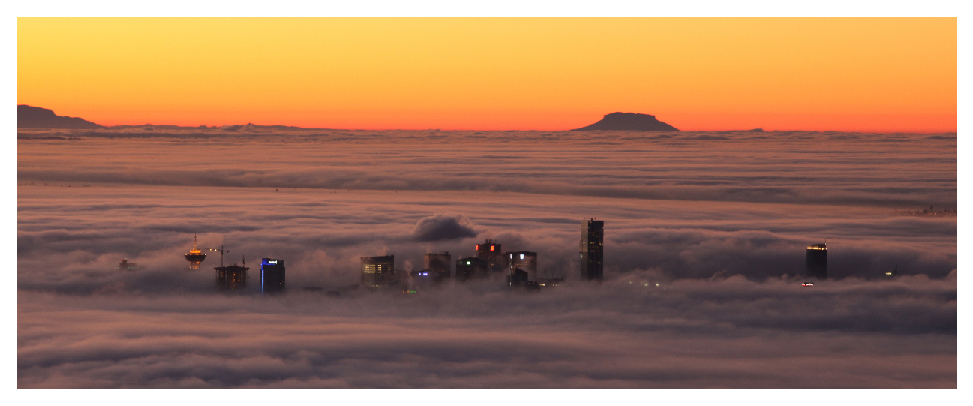
\includegraphics[width=\linewidth]{CypressView}
%  \caption{In the Clouds: Vancouver from Cypress Mountain. Note that the teaser may not be wider than the abstract block.}
%	\label{fig:teaser}
%}

%% Uncomment below to disable the manuscript note
%\renewcommand{\manuscriptnotetxt}{}

%% Copyright space is enabled by default as required by guidelines.
%% It is disabled by the 'review' option or via the following command:
% \nocopyrightspace